\subsection{Tratamiento de ruido}

\textbf{Descripción:} Se entiende por ruido a la descripción de objetos que podrían incluir
atributos basados en mediciones o juicios subjetivos, estos pueden llevar 
errores en sus valores. Otra forma de caracterizar el mismo fenómeno, consiste en
describirlo como un conjunto de individuos o registros que han sido mal clasificados.

\textbf{Metodología utilizada:} Se generó diferentes familias de datasets con ruido sobre la clase en los datos
de entrenamiento, variando desde 0\% hasta 35\%, en intervalos de 0,05\%,en los cuales
se intercambiaron los valores de la clase.
Posteriormente se ejecutó el algoritmo J48 sobre los datos de entrenamiento con los
diversos niveles ruido y con los mismos porcentajes de CF del primer experimento.
Finalmente se evaluaron los mismos con el set de validación.

\textbf{Resultados esperados:} Se espera que a medida que los niveles de ruido sobre la clase
se incrementen el tamaño del árbol aumente y la performance sobre los datos de
validación disminuya, debido a que se produce un efecto de overfitting sobre los datos de
entrenamiento.

\textbf{Análisis de los resultados}: El efecto sobre la cantidad de nodos por los diversos niveles
de ruido y poda se observan en la figura~\ref{fig:noise}a.
En el eje las abscisas se representan los
diferentes porcentajes de ruido inducido sobre la clase,
sobre el eje de ordenadas se encuentra el número de nodos del árbol.

Se observan relaciones claras entre el porcentaje de ruido y
el número de nodos del árbol,  hay incrementos 
en el tamaño del árbol a medida que el nivel de ruido incrementa.

En la figura~\ref{fig:noise}b,
se observa claramente que la presición para el 
conjunto de validación es superior a la presición del conjunto de entrenamiento 
para los valores iniciales de la función de poda, a medida que el confidence factor
aumenta, la presición del arbol se sobre ajusta al conjunto de entrenamiento.

En la figura~\ref{fig:noise}c,
Se puede observar que a medida que aumenta el porcentaje de 
ruido, la presición en el conjunto de validación disminuye drásticamente,
por lo tanto se afirma que el porcentaje de ruido inducido influye negativamente 
sobre la presición del modelo en el conjunto de validación.

En la figura~\ref{fig:noise}d,
se puede observar que la performance sobre el conjunto de validación tiene un
comportamiento muy variable con valores de CF pequeños o niveles de poda fuerte, pero
con una tendencia a disminuir a medida que el nivel de ruido aumenta. Con podas leves
o valores de CF grandes se ve con más certeza que la predicción de clases sobre el
conjunto de validación decrece a medida que aumenta el ruido.

\textbf{Conclusión:} Los niveles de ruido sobre la clase afectan el tamaño del árbol medido en
nodos, los árboles con podas severas no muestran un incremento claro en la cantidad de
nodos; sin embargo a medida que la función de poda se va flexibilizando el aumento del
tamaño del árbol se hace más evidente.

La performance sobre el conjunto de validación sufre una disminución en la predicción en
los valores de la clase cada vez que el ruido aumenta, con valores de CF bajos la
tendencia a la disminución no es muy clara; sin embargo a medida que el CF crece como
en la parte derecha de la última figura presentada en esta sección, la tendencia se
observa más fácilmente.


\begin{figure*}
  \centering
  \subfigure[Accuracy vs CF]{\label{b1} 
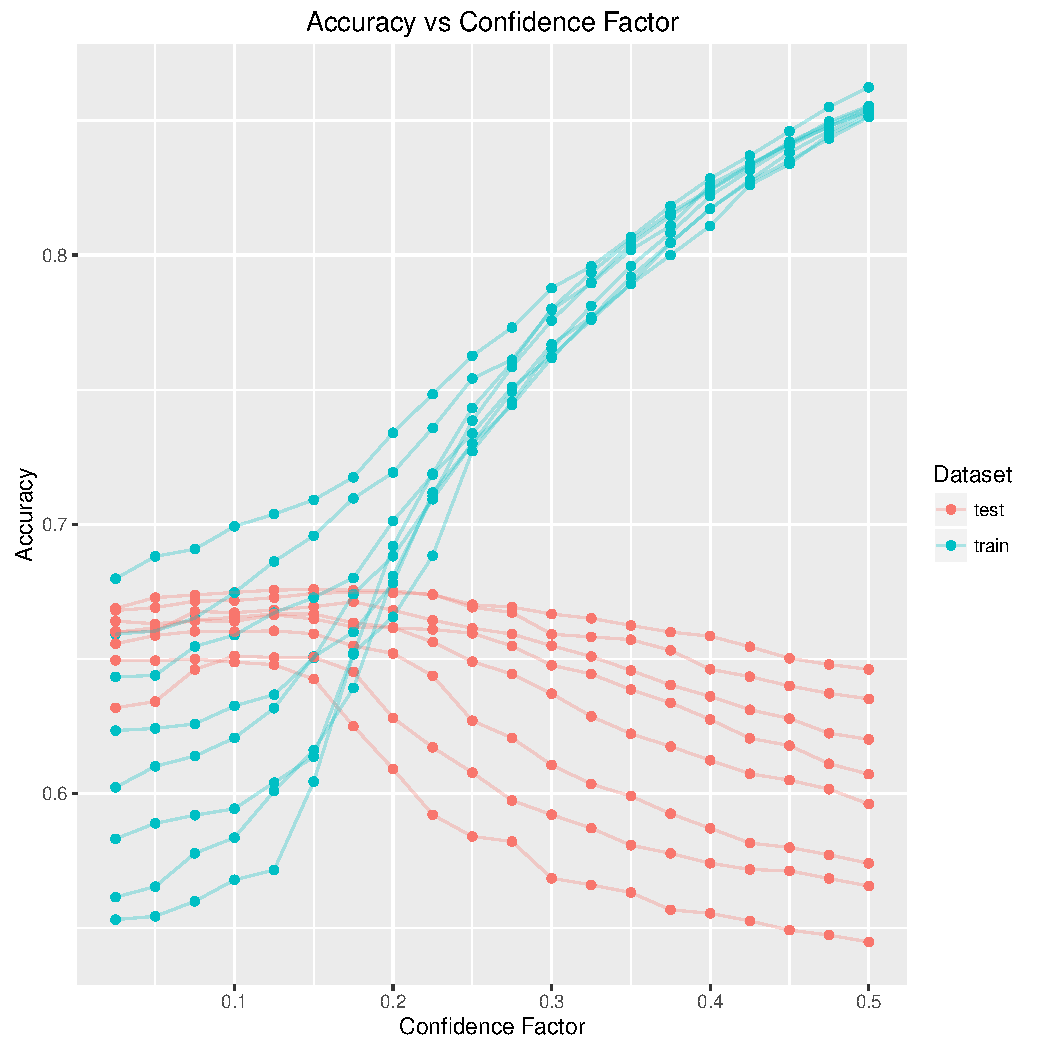
\includegraphics[width = 7cm]{5a.pdf}}
  \subfigure[Leaves vs noice percentage]{\label{b2} 
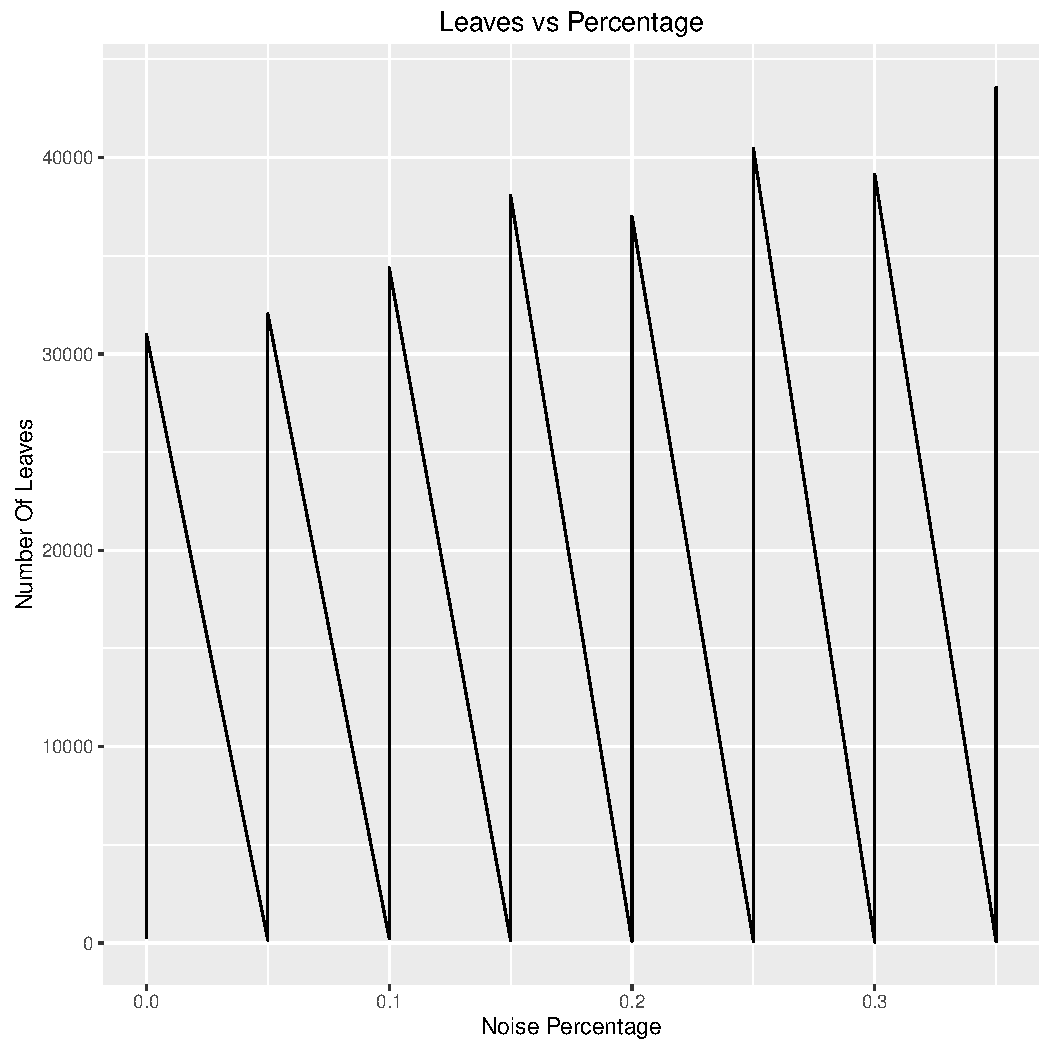
\includegraphics[width = 7cm]{5b.pdf}}
  \subfigure[Accuracy vs noise percentage]{\label{b3}
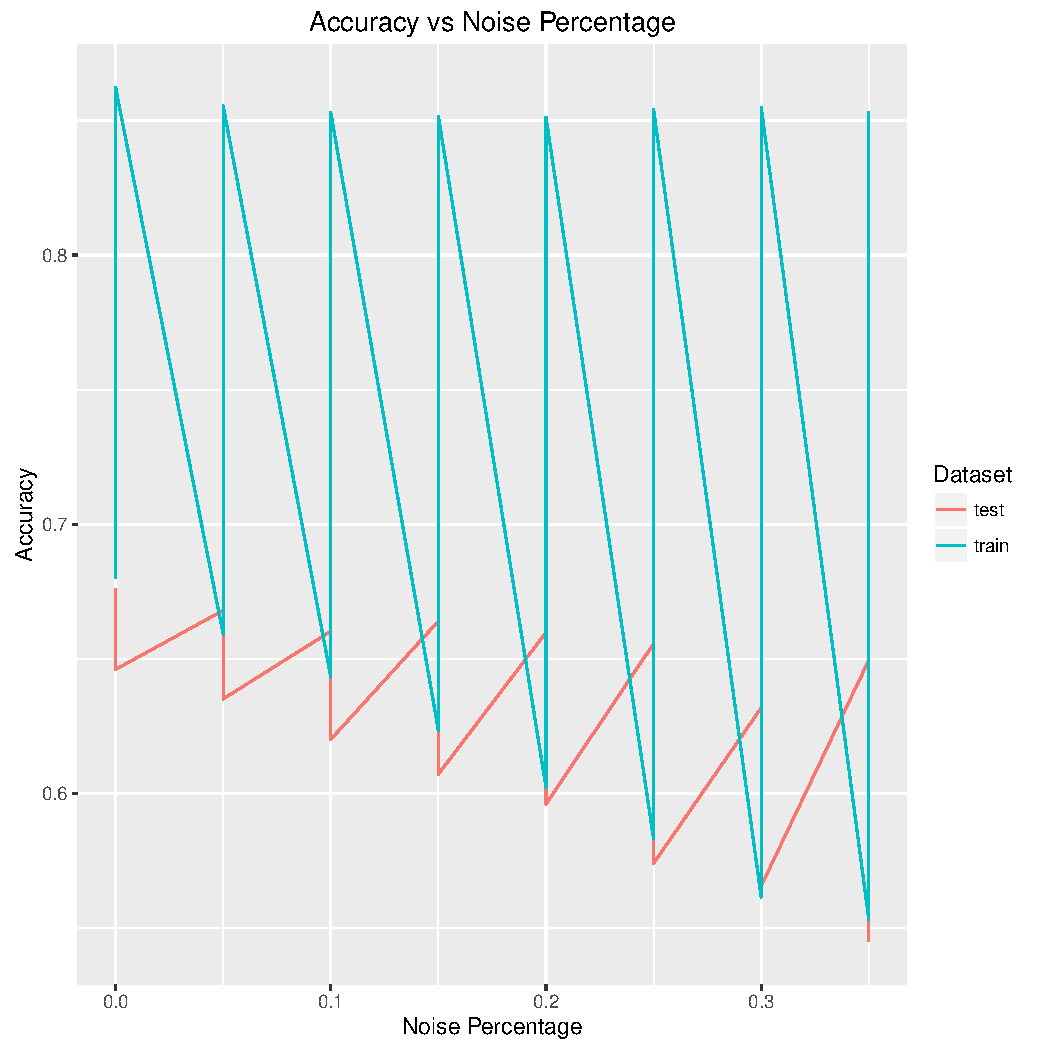
\includegraphics[width = 7cm]{5c.pdf}}
    \subfigure[Noise percentage vs CF]{\label{b4}
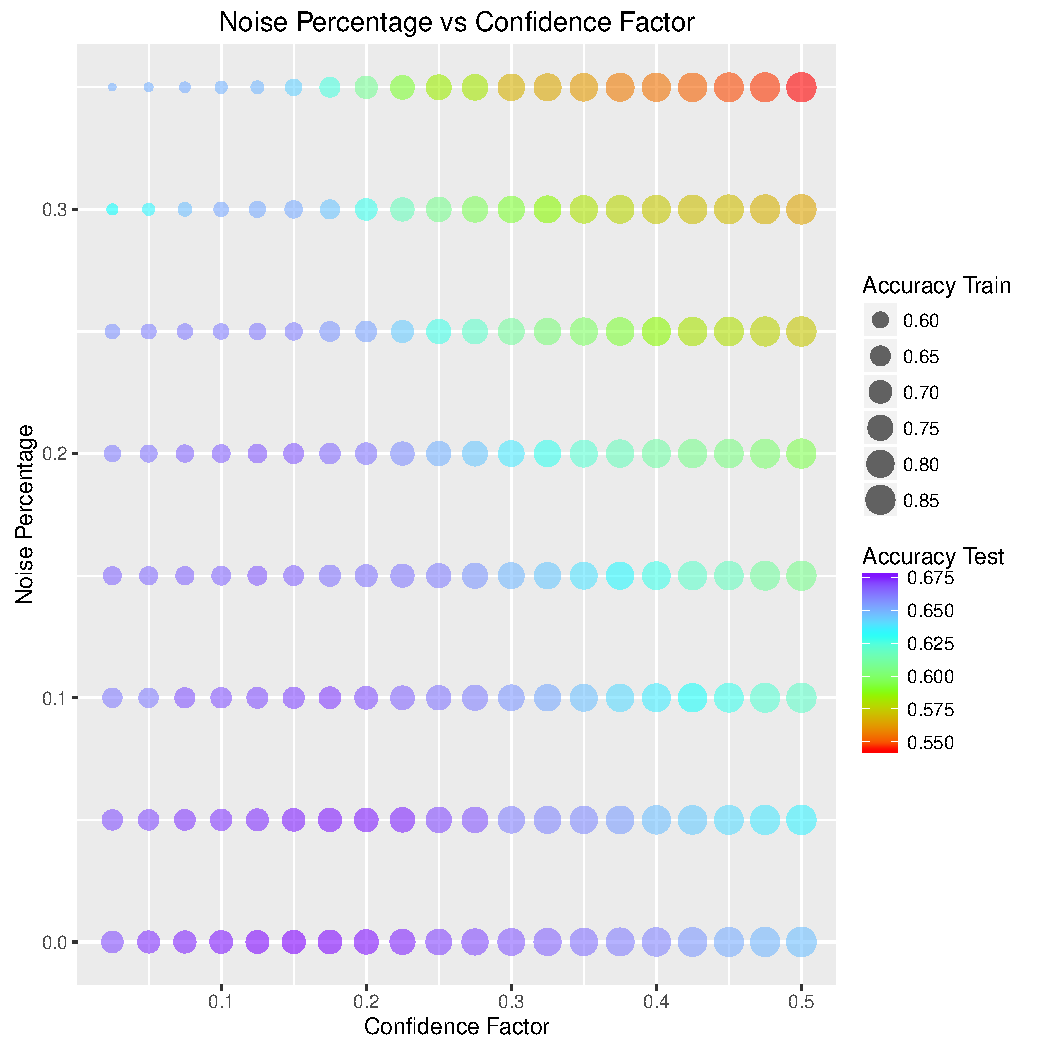
\includegraphics[width = 7cm]{5d.pdf}}
  \caption{Noise data}
  \label{fig:noise}
\end{figure*}


